\documentclass[12pt, a4paper]{article}
\usepackage[utf8]{inputenc}
\usepackage[english]{babel}
\usepackage{amsmath}
\usepackage{amsfonts}
\usepackage{amssymb}
\usepackage{siunitx}
\usepackage{longtable}
\usepackage[margin=1in]{geometry}
\usepackage{graphicx}
\usepackage{float}

\begin{document}

\begin{center}
	\Large \textbf{2: DETERMINATION OF SPECIFIC HEAT OF METALS}
	\vspace{0.5cm}
	
	\normalsize Marmara University - Department of Physics \\
	Physics 3 Laboratory \\
	Experiment Report
	\vspace{0.5cm}
\end{center}

\section{Objective}
The purpose of this experiment is to determine the specific heat capacity of iron using a calorimeter based on the principle of conservation of energy.

\section{Theoretical Background}
Heat is energy transferred due to temperature difference, while temperature is a measure of average kinetic energy.

Specific heat ($c$) is the heat required to raise 1 kg of a substance by 1°C $Q = m c \Delta T$.

According to the law of conservation of energy, total heat is conserved: $Q_{\text{received}} = Q_{\text{given}}$, so $Q_{\text{Fe}} + Q_{\text{aqua}} + Q_{\text{Cu}} = 0$.

Initially, water and copper are at equal temperature $T_1$. When hot iron is added, iron's temperature decreases from ~100°C to $T_2$, while water and copper increase to $T_2$, with heat lost by iron equaling heat gained by water and copper.

The formula is:
\[
m_{\text{Fe}} c_{\text{Fe}} (100 - T_2) = m_{\text{aqua}} c_{\text{aqua}} (T_2 - T_1) + m_{\text{Cu}} c_{\text{Cu}} (T_2 - T_1)
\]
Solving for $c_{\text{Fe}}$:
\[
c_{\text{Fe}} = \frac{(m_{\text{aqua}} c_{\text{aqua}} + m_{\text{Cu}} c_{\text{Cu}}) (T_2 - T_1)}{-m_{\text{Fe}} (T_2 - 100)}
\]

\section{Apparatus and Method}
The experiment utilized an iron sample, a calorimeter with a copper inner container, a thermometer, a stirrer, a triple beam balance, and a beaker for boiling water. The procedure involved measuring the masses of the iron, water, and copper container using the triple beam balance, heating the iron in boiling water to approximately \SI{100}{\celsius}, filling the copper container with water and measuring its mass, placing the calorimeter in an isolated environment to prevent contact between the inner and outer containers, recording the initial temperature $T_1$ with the thermometer submerged only in water, quickly transferring the heated iron into the calorimeter and stirring until thermal equilibrium was reached, then recording the final temperature $T_2$. It was noted that the iron's small mass relative to the water resulted in a minimal temperature change.

\section{Measurements and Data}
\textbf{Constants:}  
- Specific heat of water: $c_{\text{aqua}} = \SI{4200}{J/kg\celsius}$  
- Specific heat of copper: $c_{\text{Cu}} = \SI{386}{J/kg\celsius}$  
- Theoretical specific heat of iron: $c_{\text{Fe, theoretical}} = \SI{452}{J/kg\celsius}$

\begin{table}[h]
\centering
\begin{tabular}{|l|c|c|}
\hline
\textbf{Measurement} & \textbf{Symbol} & \textbf{Value} \\
\hline
Mass of iron & $m_{\text{Fe}}$ & \SI{157.9}{g} \\
Mass of water & $m_{\text{aqua}}$ & \SI{406.6}{g} \\
Mass of copper container & $m_{\text{Cu}}$ & \SI{106.5}{g} \\
Initial temperature & $T_1$ & \SI{24.1}{\celsius} \\
Final temperature & $T_2$ & \SI{27.2}{\celsius} \\
\hline
\end{tabular}
\caption{Experimental Data}
\label{tab:measurements}
\end{table}

\section{Calculations and Graphs}
\textbf{Calculations:}  
Experimental specific heat of iron:  
  \[
  c_{\text{Fe, exp}} = \frac{(\SI{0.4066}{kg} \times \SI{4200}{J/kg\celsius} + \SI{0.1065}{kg} \times \SI{386}{J/kg\celsius}) \times \SI{3.1}{\celsius}}{-\SI{0.1579}{kg} \times (\SI{27.2}{\celsius} - \SI{100}{\celsius})} = \SI{471.6}{J/kg\celsius}
  \]
Percentage error:  
  \[
  \text{Error} = \left| \frac{c_{\text{Fe, exp}} - c_{\text{Fe, theoretical}}}{c_{\text{Fe, theoretical}}} \right| \times 100 = \left| \frac{\SI{471.6}{J/kg\celsius} - \SI{452}{J/kg\celsius}}{\SI{452}{J/kg\celsius}} \right| \times 100 = 4.15\%
  \]

\textbf{Graph:}  
\begin{figure}[H]
	\centering
	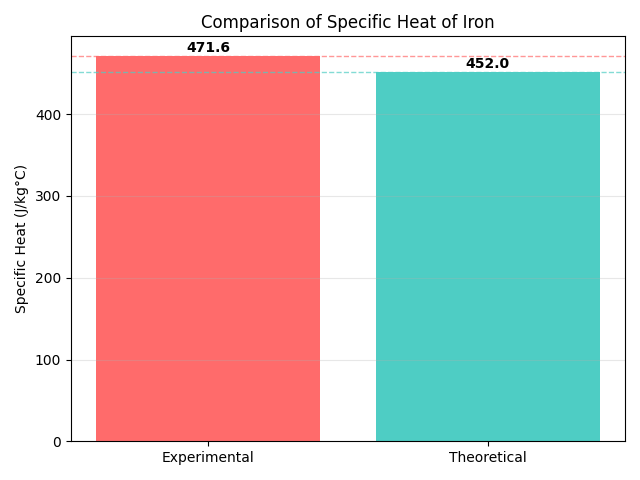
\includegraphics[width=0.6\textwidth]{Figure_1.png}
	\caption{Comparison of Specific Heat of Iron}
	\label{fig:comparison}
\end{figure}

\section{Results and Discussion}
The experimental specific heat of iron is \SI{471.6}{J/kg\celsius} compared to the theoretical value of \SI{452}{J/kg\celsius} with a 4.15\% error indicating reasonable alignment with the objective.

\textbf{Possible error sources:}  
Heat loss during iron transfer.  
Imperfect calorimeter insulation.  
Thermometer contact with non-water surfaces.

\textbf{Suggestions for improvement:} Better insulation,, larger iron mass.

\textbf{Notes:}  
Law of conservation of energy: Total $(Q_{\text{received}} = Q_{\text{given}}) = 0$, $Q_{\text{Fe}} + Q_{\text{aqua}} + Q_{\text{Cu}} = 0$.  
Initially, water and copper temperatures are equal.  
When iron is added, its temperature decreases while water and copper temperatures increase, with heat lost equaling heat gained.  
Masses measured with triple beam balance.  
Boiled water, heated iron to ~100°C.  
Transferred iron quickly to calorimeter to minimize heat loss.  
Isolated copper container, avoided outer container contact.  
Iron's small mass caused minimal water temperature change.  
Kept thermometer in water only for accuracy.  
Specific heat: Heat capacity per unit mass.  
Difference between heat and temperature: Heat is energy, temperature is a measure.

\newpage

\textbf{Student Information}

Name Surname: Hakkı Erdem Günal

Student ID: 173223024

Course: Physics 3 Laboratory

Experiment No / Title: 1 / Determination of Specific Heat of Metals

Experiment Date: October 06, 2025

Submission Date: October 12, 2025

\end{document}